\documentclass[12pt]{beamer}
\setbeamertemplate{navigation symbols}{}
\usetheme{Copenhagen}
\usepackage{listings}
\usepackage{xcolor}
\usepackage{graphicx}
\usepackage{hyperref}
\usepackage{multicol}
\graphicspath{ {imagenes/} }

\definecolor{codegreen}{rgb}{0,0.6,0}
\definecolor{codegray}{rgb}{0.5,0.5,0.5}
\definecolor{codepurple}{rgb}{0.58,0,0.82}
\definecolor{backcolour}{rgb}{0.95,0.95,0.92}

\lstdefinestyle{mystyle}{
    language=c++,
    backgroundcolor=\color{backcolour},   
    commentstyle=\color{codegreen},
    keywordstyle=\color{magenta},
    numberstyle=\tiny\color{codegray},
    stringstyle=\color{codepurple},
    basicstyle=\ttfamily\footnotesize,
    breakatwhitespace=false,         
    breaklines=true,                 
    captionpos=b,                    
    keepspaces=true,                 
    numbers=left,                    
    numbersep=5pt,                  
    showspaces=false,                
    showstringspaces=false,
    showtabs=false,                  
    tabsize=2
}

\lstset{style=mystyle}

\title{Archivos}
\subtitle{Archivos de texto}
\author{Tomás Peiretti}
\date{}

\begin{document}

\maketitle

\begin{frame}{Archivos de texto}
    Puntos clave:
    \begin{itemize}
        \item La información se almacena como una secuencia de caracteres.
        \item Son secuenciales: El orden de acceso a los datos está determinado, primero se accede al primer elemento y luego se puede ir accediendo a los siguientes, de uno en uno.
        \item Hay 3 tipos:
        \begin{itemize}
            \item De entrada: \alert{ifstream}
            \item De salida: \alert{ofstream}
            \item De entrada/salida: \alert{fstream}
        \end{itemize}
    \end{itemize}
\end{frame}

\begin{frame}{Archivos de texto: implementación}
    Para utilizar un archivo de texto en nuestro programa debemos:
        \begin{enumerate}
            \item Incluir la librería fstream
            \item Declarar la variable que actuará como manejador de fichero
            \item Abrir el flujo de datos, vinculando la variable correspondiente con el fichero especificado.
            \item Comprobar que la apertura del fichero se realizó correctamente
            \item Realizar la transferencia de información
            \item Finalmente, cerrar el flujo para liberar la variable manejador de su vinculación con el fichero.
        \end{enumerate}
\end{frame}

\begin{frame}[fragile]{Archivos de texto: implementación}
\begin{lstlisting}[basicstyle=\scriptsize]
#include <iostream>
#include <fstream>  //1
using namespace std;

int main(int argc, char *argv[]) {
	ifstream archivo; // 2
	archivo.open("text.txt"); // 3
	
	if (archivo.is_open()) { // 4
		int x;
		archivo >> x; // 5
		cout << "Valor en el archivo = " << x << endl;
	}
	else {
		cout << "Error al abrir el archivo" << endl;
	}
	
	archivo.close(); // 6
	
	return 0;
}
\end{lstlisting}
\end{frame}

\begin{frame}{Archivos de texto: modos de apertura}
    Para abrir un archivo siempre utilizaremos el método \alert{open}, el cual recibe 2 parámetros:
    \begin{itemize}
        \item El nombre del archivo a abrir
        \item El modo de apertura
    \end{itemize}
    \medskip
    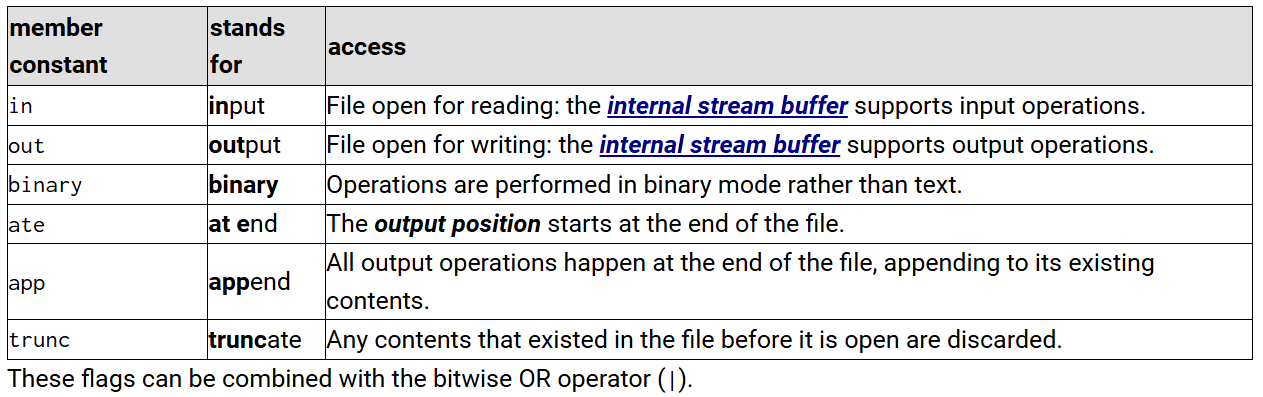
\includegraphics[width=\textwidth]{modos-apertura.png}
\end{frame}

\begin{frame}[fragile]{Archivos de texto: ejemplo}
    \begin{lstlisting}[basicstyle=\tiny]
// Ejemplo: de un archivo que almacena numeros enteros,
// se debe procesar e imprimir la suma de todos ellos
int main() {
    fstream arch;
    arch.open("numeros.txt", ios::in);
    
    if (arch.is_open()) {
        int x;
        int sum = 0;
        while (arch >> x) {
            sum += x;
        }
        cout << sum << endl;
    }
    else {
        cout << "Error al abrir el archivo" << endl;
    }
    
    arch.close();
    
    return 0;
}
\end{lstlisting}
\end{frame}

\begin{frame}[fragile]{Archivos de texto: ejemplo}
\begin{lstlisting}[basicstyle=\tiny]
// Ejemplo: de un archivo que almacena numeros enteros,
// se debe procesar e imprimir la suma de todos ellos
int main() {
	fstream arch;
	arch.open("numeros.txt", ios::in);
	
	if (arch.is_open()) {
		int x;
		int sum = 0;
		while (arch >> x) {
			sum += x;
		}
		cout << sum << endl;
	}
	else {
		cout << "Error al abrir el archivo" << endl;
	}
	
	arch.close();
	
	return 0;
}
\end{lstlisting}
\begin{itemize}
    \item Un archivo de texto de entrada se comporta igual que \alert{cin}
    \item Un archivo de texto de salida se comporta igual que \alert{cout}
\end{itemize}
\end{frame}

\end{document}